\documentclass{beamer}

\usepackage{tikz}
\usetikzlibrary{decorations.pathreplacing}
\usepackage{mathtools}
\usepackage{graphicx}

\AtBeginDocument{\newcommand{\im}{\textnormal{i}}}

% Tema da apresentação
\usetheme{Madrid} % Outros temas: AnnArbor, Copenhagen, Dresden, Warsaw, etc.

\newcommand{\lastframetitle}{}

% Atualiza o título do último slide em cada frame
\addtobeamertemplate{frametitle}{}{\xdef\lastframetitle{\insertframetitle}}

% \AtBeginSection[]{
%     \addtocounter{framenumber}{-1}
%   \begin{frame}{Sumário}
%     \tableofcontents[currentsection] % Destaca a seção atual
%   \end{frame}
    
% }

\useoutertheme{split}
\setbeamertemplate{headline}{%
  \leavevmode%
  \hbox{%
    \begin{beamercolorbox}[wd=0.5\paperwidth,ht=2.5ex,dp=1ex,left]{section in head/foot}%
      \hspace{1em}\insertsectionhead
    \end{beamercolorbox}%
    \begin{beamercolorbox}[wd=0.5\paperwidth,ht=2.5ex,dp=1ex,left]{subsection in head/foot}%
      \hspace{1em}\ifx\insertframetitle\empty
      \lastframetitle % Mostra o último título válido
    \else
    \fi
    \end{beamercolorbox}%
  }
  \vskip0pt%
}

\setbeamertemplate{footline}{%
  \leavevmode%
  \hbox{%
    % Caixa da esquerda: autor
    \begin{beamercolorbox}[wd=0.33\paperwidth,ht=2.5ex,dp=1ex,left]{author in head/foot}%
      \hspace{1em}\insertauthor
    \end{beamercolorbox}%
    % Caixa da direita: título da apresentação
    \begin{beamercolorbox}[wd=0.67\paperwidth,ht=2.5ex,dp=1ex,right]{title in head/foot}%
      \inserttitle\ \ \insertframenumber{} / \inserttotalframenumber\hspace{1em}
    \end{beamercolorbox}%
  }
  \vskip0pt%
}



% Pacotes adicionais
\usepackage[utf8]{inputenc} % Codificação UTF-8
\usepackage[brazil]{babel} % Língua portuguesa do Brasil
\usepackage{graphicx} % Para inserir imagens
\usepackage{amsmath,amssymb} % Para matemática avançada
\usepackage{physics}
\usepackage{tensor}
\usepackage{bbm}
\usepackage{mathtools}

\usefonttheme{serif}

% Informações da apresentação
\title{A Modelagem Científica vista como um Campo Conceitual}
\author{Brandão, Araujo \& Veit (2011)}
\institute{Vicente Viater Figueira}
\date{\today}

\begin{document}

\frame{\titlepage}

\section{Introdução}

\begin{frame}{Resumo}
\begin{itemize}
    \item DOI: 10.5007/2175-7941.2011v28n3p507
\end{itemize}
\begin{block}{Brandão, Araujo \& Veit (2011)}
Este  trabalho  defende  a  tese  de  que  o  processo  de  modelagem  científica em  
Física  pode  ser  visto  como  um  campo  conceitual  sub-jacente  ao  domínio  de  
campos  conceituais  específicos  dessa  ciência  e  possui  implicações  relevantes  
para  o  seu  ensino  e  pesquisa.  Para tanto, apoia-se na visão epistemológica de 
\textbf{Mario Bunge} sobre modelagem científica e na \textbf{Teoria dos Campos Conceituais} de \textbf{Gérard  
Vergnaud},  levando  em  conta  as  ideias  de  Weil-Barais  e  Vergnaud sobre concepções em Física.
\end{block}
\end{frame}

\section{Fundamentos Teóricos}
\begin{frame}{Modelagem Científica segundo Mario Bunge}
\begin{itemize}
    \item Objeto-Concreto $\Rightarrow$ Objeto-Modelo
    \item Teoria-Geral
\end{itemize}
\vspace{2em}
\begin{itemize}
    \item Teoria-Geral $+$ Objeto-Concreto $\Rightarrow$ Teoria-Específica
\end{itemize}
\vspace{2em}
\begin{itemize}
    \item ``...Por fim, na medida em que todo modelo teórico é, em certo grau, 
    uma invenção, sua falseabilidade deve estar constantemente sendo avaliada...''
\end{itemize}
\end{frame}

\begin{frame}{TCC de Gérard Vergnaud}
\begin{itemize}
    \item Construção de Conhecimento nunca é isolada
\end{itemize}
\vspace{2em}
\begin{itemize}
    \item Conceitos-em-ação
    \item Teoremas-em-ação
    \item Esquemas
\end{itemize}
\vspace{2em}
\begin{itemize}
    \item Construção de conhecimento científico é explicitação destes
\end{itemize}
\end{frame}

\section{Modelagem Científica como Campo Conceitual}
\begin{frame}{Estrutura Conceitual de Referência}
    \begin{figure}
        \centering
        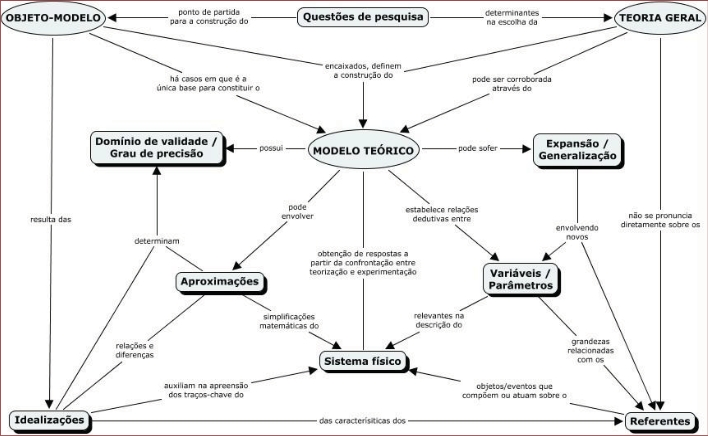
\includegraphics[width=\linewidth]{TCCModel.jpeg}
    \end{figure}
\end{frame}

\section{Implicações para o Ensino de de Física}

\begin{frame}{Conclusões}
\begin{itemize}
    \item Situações problema altamente idealizadas desconexas da realidade.
    \item Estímulo à construção ativa do conhecimento.
    \item Desenvolvimento do pensamento científico e crítico.
\end{itemize}
\vspace{2em}
\begin{itemize}
    \item ``...como eu devo responder a essas questões? De acordo com o que você nos ensinou, ou da forma como eu penso sobre essas coisas?...''
\end{itemize}
\end{frame}

\begin{frame}{Referências}
Brandão, R. V., Araujo, I. S., \& Veit, E. A. (2011). \textit{A modelagem científica vista como um campo conceitual}. Caderno Brasileiro de Ensino de Física, 28(3), 507–545. \\
\href{https://periodicos.ufsc.br/index.php/fisica/article/view/2175-7941.2011v28n3p507}{Link para o artigo}
\end{frame}

% \addtocounter{framenumber}{2000}

\end{document}